\chapter{Método y Fases de Trabajo}
\label{chap:metodologia}

\drop{C}on el fin de hacer más comprensible al lector el proceso de desarrollo, cómo se ha planificado y llevado a cabo, en este capítulo se aportarán los conceptos básicos que rodean a la metodología empleada y se describirán las herramientas utilizadas, intentado dar una visión general de la misma y su aplicación en el proyecto.

\section{Metodología}

La elección de una metodología acertada es fundamental para que el desarrollo del proyecto que se tiene entre manos llegue a buen puerto. Para ello es muy importante tener en cuenta aquellas metodologías que mejor se adapten a nuestros conocimientos, estado del arte, lenguajes de programación y los plazos de tiempo que se tendrán, así como el entorno (físico y digital) en el que se llevará a cabo el desarrollo e implantará la solución. 

Por estos motivos a la hora de tomar una decisión, analicé las características más importantes de los dos grupos de metodologicos existentes, con el fin de aplicar la mejor solución al desarrollo de este proyecto.

\subsubsection{Metodologías tradicionales}

Son aquellas que basándose en una especificación precisa de los requisitos y en el modelado, se centran más en la planificación y en el control del proyecto. Con carácter general la aplicación de este tipo de metodologías requiere conocer no solo con exactitud el alcance del trabajo a llevar a cabo, también es necesario antes de teclear una sola línea de código, planificar completamente todas las fases del desarrollo del proyecto (ver Figura~\ref{fig:modelo-en-cascada}). Estas metodologías no se adaptan adecuadamente a los cambios en los requisitos del proyecto y no son muy útiles cuando no se conoce el alcance de todo lo que se quiera o necesite hacer.

\begin{figure}[h]
\centering
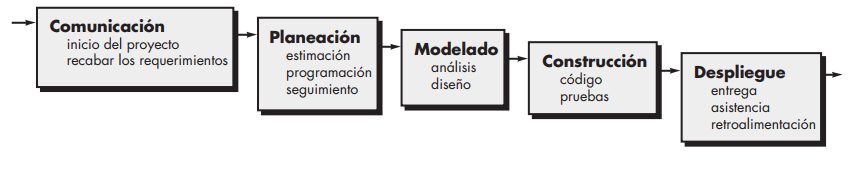
\includegraphics[width=1\textwidth]{/modelo_cascada.png}
\caption{Etapas del Modelo en cascada~\cite{iso_enfoque_practico}}
\label{fig:modelo-en-cascada}
\end{figure}

\subsubsection{Metodologías ágiles}

Surgen como respuesta a los inconvenientes que trae consigo el desarrollo de software tradicional, donde el trabajo comienza con la construcción de una extensa documentación en la que se recogen, los requisitos del sistema (funcionales\footnote{\url{https://es.wikipedia.org/wiki/Requisito_funcional}} y no funcionales\footnote{\url{https://es.wikipedia.org/wiki/Requisito_no_funcional}}), seguida del diseño minucioso de la arquitectura, una completa descripción del proceso de desarrollo y otros. 

En 2001, Kent Beck\footnote{\url{https://www.linkedin.com/in/kentbeck}} y otros 16 notables, desarrolladores de software, consultores y editores, firmaron el «\textit{Manifiesto por el desarrollo ágil de software}»\footnote{\url{http://agilemanifesto.org/iso/es/manifesto.html}} y en él se dice lo siguiente:

\begin{quote}
{\itshape

Estamos descubriendo formas mejores de desarrollar software tanto por nuestra propia experiencia como ayudando a terceros. A través de este trabajo hemos
aprendido a valorar:
\begin{itemize}
\item\textbf{Individuos e interacciones} sobre procesos y herramientas
\item \textbf{Software funcionando} sobre documentación extensiva
\item \textbf{Colaboración con el cliente} sobre negociación contractual
\item \textbf{Respuesta ante el cambio} sobre seguir un plan
\end{itemize}

Esto es, aunque valoramos los elementos de la derecha, valoramos más los de la izquierda.
}
\par\nointerlineskip\noindent\hfill Manifiesto por el desarrollo ágil de software~\cite{AgileManifest}
\end{quote}

\subsubsection{Recursos disponibles}
Debido a las siguientes limitaciones:

\begin{itemize}
\item Situación laboral: Sólo me permitía asignarle un tiempo bastante irregular al desarrollo del proyecto y su documentación. Además restringía bastante la frecuencia de las tutorías en persona con los inconvenientes que ello conllevaba.
\item Naturaleza del proyecto: No solo no estaba claro que lenguaje emplear dado que el proyecto se basa en una aplicación web, tampoco estaban muy bien definidos todos los requisitos y el alcance de los problemas que abordaría o solventaría la aplicación.
\end{itemize}

Me he decantado por el uso de un «\textit{desarrollo evolutivo}» que me permitiese abordar el proyecto de la forma más organizada posible y que mostrase el potencial de la aplicación desde el primer instante. De esta forma podría ir desarrollando el software conforme a las pautas establecidas y en caso de que se fuesen modificando lo requisitos, o si surgiesen nuevas necesidades no tenidas en cuenta desde un primer momento, se pudiesen incorporar al desarrollo con el menor costo e impacto posible.

\subsection{Prototipado evolutivo}

Dadas las circunstancias vistas anteriormente, se ha optado por el uso de «\textit{prototipado evolutivo}», la metodología más ágil de las tradicionales, en cuanto a que se plantea la consecución del sistema en su totalidad a través del desarrollo de prototipos (ver Figura~\ref{fig:evolutivo}). 

Algunos autores consideran que el prototipado evolutivo no debería ser enmarcado dentro de las metodologías de prototipado, sino como una metodología que trata con el desarrollo de versiones, es decir, una estrategia a seguir que ve el producto como una secuencia de versiones a evaluar y que sirven como prototipo para versiones posteriores~\cite{floy_prot}.

\begin{figure}[h]
\centering
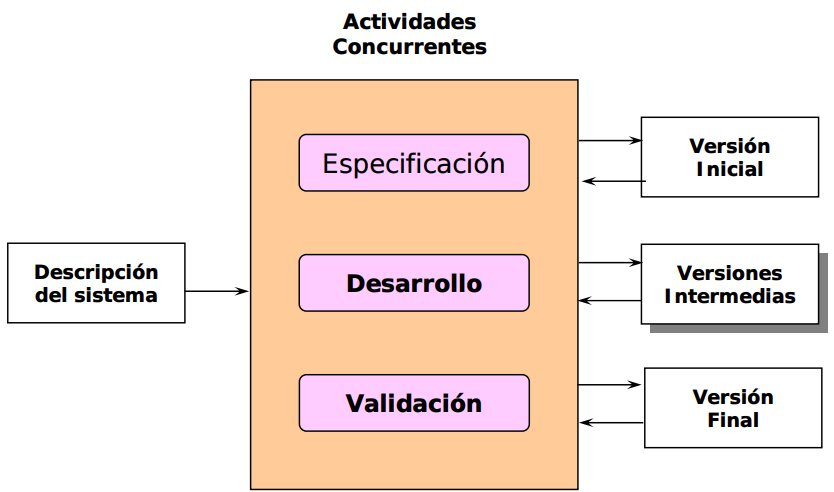
\includegraphics[width=1\textwidth]{/evolutivo.png}
\caption{Modelo Evolutivo~\cite{Evolutivo}}
\label{fig:evolutivo}
\end{figure}

Como en nuestro caso no tenemos claro el alcance del proyecto en su totalidad, resulta incómodo y poco práctico el uso estricto de las fases de \textbf{análisis}, \textbf{diseño}, \textbf{construcción}, \textbf{evaluación} y \textbf{refinado} (ver Figura~\ref{fig:proto}). En vez de eso se suavizarán cada una de las fases y se irán desarrollando con una frontera no tan definida y con la particularidad de volver atrás en cualquier momento, sin necesidad de tener que llegar a la fase de \textbf{evaluación} con la \textbf{construcción} del prototipo finalizada.

\begin{figure}[!h]
\centering
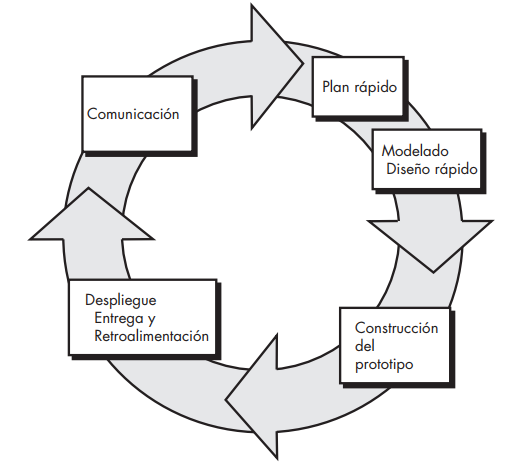
\includegraphics[width=0.7\textwidth]{/proto.png}
\caption{El paradigma en la construcción de prototipos~\cite{floy_prot}}
\label{fig:proto}
\end{figure}

\section{Fases de Trabajo}
\label{sec:fasesdetrabajo}

En esta sección se describen las iteraciones para la consecución parcial o total de los prototipos de nuestro proyecto. Como es de esperar en la primera fase o iteración de desarrollo no tendremos un prototipo, sino que nos centraremos en satisfacer todos los requisitos no vinculados específicamente con la funcionalidad del proyecto pero que sí son determinantes para su consecución satisfactoria. En las siguientes iteraciones se irán obteniendo prototipos que pasarán de ser parciales a completos y que nos ayudarán a definir exactamente aquellos requisitos funcionales que no se identificaron a primera vista y no están completamente claros.

\subsection{Iteración 0}
\label{sub:metodologiaiter0}

Como ya se ha comentado en el apartado anterior, antes de llegar a tener el primer prototipo completado es necesario hacer frente a ciertos factores que condicionarán la evolución y el desarrollo del proyecto en gran media, los requisitos no funcionales y funcionales. Para ello es necesario:

\begin{itemize}
\item Buscar información acerca de la normativa de seguridad privada en nuestro país.
\item Analizar e indagar en los sistemas de seguridad para sacar sus principales componentes y funcionalidades.
\item Investigar las soluciones comerciales de bajo coste y extraer de los mismos ideas y tendencias.
\item Elección de un marco de desarrollo apropiado.
\item Extracción de requisitos de lo que sería un sistema muy básico.
\end{itemize}

\subsection{Iteración 1}
\label{sub:metodologiaiter1}

El objetivo de esta iteración es la familiarización con el entorno de desarrollo a través de la puesta en práctica de tutoriales y ejemplos, contextualizados dentro de lo posible en el ámbito de la seguridad. Para ello se han planteado los siguentes aspectos a cubrir:

\begin{itemize}
\item Búsqueda de ejemplos de explotación y uso de la librerías en \hyperref[tab:arduino-yun]{\textit{Arduino-Yún}}.
\item Desarrollo de ejemplos con \hyperref[tab:arduino-yun]{\textit{Arduino-Yún}} para evaluar su validez de aplicación en el proyecto.
\item Desarrollo de una maqueta que explote las funcionalidades añadidas que ofrece \hyperref[tab:arduino-yun]{\textit{Arduino-Yún}}.
\end{itemize}

\subsection{Iteración 2}
\label{sub:metodologiaiter2}

En esta iteración se persigue conseguir un método factible para emular el comportamiento aproximado que pudiese tener nuestra controladora de dispositivos. Esto se hace de esta manera para facilitar el desarrollo y pruebas del sistema, sin necesidad de tener que afinar todos los aspectos que requiere el hardware real con la penalización temporal que ello conlleva.
 
\begin{itemize}
\item Desarrollo software de un sistema \textit{dummy}\footnote{Fake, not real. Que es falso, no real.} que emule el comportamiento real de una controladora con sus detectores.
\item Implementación de un método que facilite la prueba de comportamientos o estados específicos en el sensor.
\item Visualización por consola de los eventos que se van produciendo. 
\end{itemize}

\subsection{Iteración 3}
\label{sub:metodologiaiter3}

Tras haberse planteado en la iteración anterior un sistema de emulación de señales, el siguiente punto propuesto es crear la aplicación web que pueda explotarlo y sacar un mínimo de funcionalidad al mismo. Para ello en esta iteración se pretenden:

\begin{itemize}
 \item Desarrollar los mecanismos CRUD para operar sobre los modelos necesarios en nuestra interfaz de administración en el \textit{backend}\footnote{Capa de acceso y edición de los datos en el servidor.}.
 \item Creación de un log de eventos, con la capacidad de filtrar la información contenida en nuestra \acs{BBDD}, de una forma simple he intuitiva.
 \item Creación de un método de aprovisionamiento para alimentar la \acs{BBDD} con aquellos datos que puedan resultar útiles para establecer un punto de partida en el uso de la herramienta.
 \end{itemize}

\subsection{Iteración 4}
\label{sub:metodologiaiter4}
En esta iteración es donde se tiene por objetivo completar lo que sería la arquitectura del sistema, desde la controladora hardware hasta la aplicación que utiliza el usuario para supervisar los eventos. Teniendo en cuanta todo el desarrollo hasta el momento, la idea anterior y la necesidad de que el sistema permita acoger la integración de nuevos dispositivos y funcionalidades con poco o ningún esfuerzo, podemos resumir las tareas de esta iteración en:

\begin{itemize}
\item Desarrollar una \acs{API}-\acs{REST} que permita la creación de eventos así como la consulta de información y parámetros relativos al sistema.
\item Adaptar el sistema de emulación para que utilice y aproveche la nueva \acs{API}-\acs{REST} obteniendo funcionamientos más complejos como la emisión solo de nuevos estados físicos y no de los mismos una y otra vez, para no llenar la \acs{BBDD} de eventos que no aportan ninguna información nueva.

\end{itemize}

\subsection{Iteración 5}
Tras haber completado la arquitectura de nuestra aplicación en la iteración anterior, salen a la luz necesidades que han quedado relegadas a las fases posteriores del desarrollo del proyecto, como pueden ser:

\begin{itemize}
\item Mejora de la usabilidad del sistema, mediante el uso de iconos.
\item Creación de un método de autenticación de los usuarios y validación de los datos del formulario de \textit{login}\footnote{\url{https://es.wikipedia.org/wiki/Login}}.
\item Uso exclusivo de la \acs{API}-\acs{REST} para aquellos usuarios que dispongan de las credenciales autorizadas para hacerlo.
\end{itemize} 

\section{Herramientas}

En este apartado se describen las herramientas utilizadas para el desarrollo del proyecto (documentación y aplicación).

\subsection{Aplicaciones utilizadas}

\begin{definitionlist}
\item[Light Table:] Editor de texto \textit{open source}\footnote{\url{https://en.wikipedia.org/wiki/Open-source_model}}, muy similar a \textit{Sublime Text}\footnote{\url{https://www.sublimetext.com/}}, con numerosos \textit{plugins} a disposición de la comunidad~\cite{Lighttable}. Se ha utilizado para la edición de la mayor parte del código y documentación aportada.
\item[\acs{GNU} Nano:] Editor de texto por consola ligero, pequeño, gratuito y del tipo \textit{Software Libre}. Viene disponible por defecto en prácticamente todas las distribuciones del sistema operativo \textit{Ubuntu}\footnote{\url{https://www.ubuntu.com/}} y se puede encontrar en todos los repositorios \textit{Debian}\footnote{\url{https://www.debian.org/index.es.html}} oficiales~\cite{Nano}. Se ha utilizado puntualmente para la edición de algún \textit{Makefile}\footnote{\url{https://www.gnu.org/software/make/manual/make.html}} y para plasmar el contenido de los \textit{commits}\footnote{\url{https://www.mercurial-scm.org/repo/hg/help/commit}} del repositorio \textit{Mercurial}
\item[Mercurial:] Sistema de control de versiones distribuido. Se ha hecho uso de esta herramienta para el código del proyecto y la documentación~\cite{Mercurial}.
\item[\acs{GIMP}:] Programa libre y gratuito para la edición de imágenes en forma de mapa de bits~\cite{Gimp}. Se ha utilizado para editar algunas de las imágenes existentes en esta documentación.
\item[Arduino \acs{IDE}:] \textit{Software} \textit{open source} que facilita la creación, edición y subida de código a cualquiera de las placas de la familia Arduino~\cite{ArduinoIDE}.

\end{definitionlist}


\subsection{Lenguajes de programación, entornos y librerías}

\begin{definitionlist}
\item[Python:] Lenguaje de programación interpretado, con tipado dinámico, multiplataforma y multiparadigma ya que soporta orientación a objetos, programación imperativa y, en menor medida, programación funcional~\cite{Python}.
\item[Django:] \textit{Framework}\footnote{\url{https://en.wikipedia.org/wiki/Software_framework}} Web \textit{open source} de alto nivel basado en Python que fomenta un desarrollo rápido y un diseño limpio~\cite{Django}.
\item[Django \acs{REST} \textit{Framework}:] Es un conjunto de herramientas potentes y flexibles pensadas para crear \acs{API}s web~\cite{RestFramework}.
\item[Django-Rest-Auth:] Librería que proporciona las funcionalidades básicas de autenticación como, \textit{login}, \textit{logout} y cambio de contraseña a \textit{Django} \acs{REST} \textit{Framework}~\cite{RestAuth}.
\item[AngularJS:] \textit{Framework} \textit{JavaScript}\footnote{\url{https://www.javascript.com/}} de código abierto mantenido por Google\footnote{\url{https://www.google.es/intl/es/about/}} ideal para declarar vistas dinámicas en aplicaciones web~\cite{AngularJS}.
\item[\acs{HTML5}:] Quinta versión del lenguaje de marcado más importante de la \textit{World Wide Web}\footnote{\url{https://es.wikipedia.org/wiki/World_Wide_Web}}~\cite{HTML5}.
\item[\acs{CSS3}:] Versión 3 \acs{CSS}, lenguaje usado para definir la representación de un documento estructurado escrito en \acs{HTML}~\cite{CSS3}.
\item[Zero C-Ice:] Marco completo \acs{RPC}, con soporte para C++, C\#, Java, JavaScript, Python y más lenguajes~\cite{ZeroC}.
\item[\LaTeX:] Lenguaje de marcado de documentos de carácter técnico y científica, utilizado para realizar este documento~\cite{Latex}.
\end{definitionlist}


\subsection{Sistemas Operativos}

\begin{definitionlist}

\item[Debian:] Sistema operativo libre que actualmente usa el núcleo de \textit{Linux}\footnote{\url{https://www.kernel.org/}} o \textit{FreeBSD}\footnote{\url{https://www.freebsd.org/}}~\cite{Debian}. Se ha empleado para soportar todo el conjunto de programas, herramientas y aplicaciones descritas anteriormente incluidos los propios prototipos generados en el desarrollo (ver Listado~\ref{code:debian_version}).

\item[OpenWrt-Yun:] Distribución del sistema operativo \textit{Linux}\footnote{\url{https://en.wikipedia.org/wiki/Linux_kernel}}, instalado por defecto en la placa Arduino-Yún, basado en \textit{OpenWrt}\footnote{\url{https://openwrt.org/}}, que permite la configuración del sistema a través de línea de comandos~\cite{Arduino-Yun}.
\end{definitionlist}

\lstinputlisting[label = {code:debian_version}, caption = {Versión del sistema operativo del portátil de desarrollo}, style = customconsole]{code/debian_version.console}


\subsection{Hardware}
\begin{definitionlist}
\item[Ordenador portátil:] Para el desarrollo del proyecto se ha utilizado un portátil marca ACER, modelo ASPIRE 5755G, con un procesador Intel$^{(R)}$ Core$^{TM}$ I7-2670QM a 2.2GHz, 4GB DDR3 de memoria \acs{RAM} y 1TB de disco duro.

\item[Arduino:] Para las pruebas de librerías de Arduino y la realización de ejemplos y prototipos que sirviesen de ejemplo para la construcción de nuestra controladora hardware, se ha utilizado una placa \hyperref[tab:arduino-yun]{\textit{Arduino-Yún}} (\hyperref[chap:anexo3]{ver Anexo~\ref{chap:anexo3}}).
\end{definitionlist}
